\documentclass[1p]{elsarticle_modified}
%\bibliographystyle{elsarticle-num}

%\usepackage[colorlinks]{hyperref}
%\usepackage{abbrmath_seonhwa} %\Abb, \Ascr, \Acal ,\Abf, \Afrak
\usepackage{amsfonts}
\usepackage{amssymb}
\usepackage{amsmath}
\usepackage{amsthm}
\usepackage{scalefnt}
\usepackage{amsbsy}
\usepackage{kotex}
\usepackage{caption}
\usepackage{subfig}
\usepackage{color}
\usepackage{graphicx}
\usepackage{xcolor} %% white, black, red, green, blue, cyan, magenta, yellow
\usepackage{float}
\usepackage{setspace}
\usepackage{hyperref}

\usepackage{tikz}
\usetikzlibrary{arrows}

\usepackage{multirow}
\usepackage{array} % fixed length table
\usepackage{hhline}

%%%%%%%%%%%%%%%%%%%%%
\makeatletter
\renewcommand*\env@matrix[1][\arraystretch]{%
	\edef\arraystretch{#1}%
	\hskip -\arraycolsep
	\let\@ifnextchar\new@ifnextchar
	\array{*\c@MaxMatrixCols c}}
\makeatother %https://tex.stackexchange.com/questions/14071/how-can-i-increase-the-line-spacing-in-a-matrix
%%%%%%%%%%%%%%%

\usepackage[normalem]{ulem}

\newcommand{\msout}[1]{\ifmmode\text{\sout{\ensuremath{#1}}}\else\sout{#1}\fi}
%SOURCE: \msout is \stkout macro in https://tex.stackexchange.com/questions/20609/strikeout-in-math-mode

\newcommand{\cancel}[1]{
	\ifmmode
	{\color{red}\msout{#1}}
	\else
	{\color{red}\sout{#1}}
	\fi
}

\newcommand{\add}[1]{
	{\color{blue}\uwave{#1}}
}

\newcommand{\replace}[2]{
	\ifmmode
	{\color{red}\msout{#1}}{\color{blue}\uwave{#2}}
	\else
	{\color{red}\sout{#1}}{\color{blue}\uwave{#2}}
	\fi
}

\newcommand{\Sol}{\mathcal{S}} %segment
\newcommand{\D}{D} %diagram
\newcommand{\A}{\mathcal{A}} %arc


%%%%%%%%%%%%%%%%%%%%%%%%%%%%%5 test

\def\sl{\operatorname{\textup{SL}}(2,\Cbb)}
\def\psl{\operatorname{\textup{PSL}}(2,\Cbb)}
\def\quan{\mkern 1mu \triangleright \mkern 1mu}

\theoremstyle{definition}
\newtheorem{thm}{Theorem}[section]
\newtheorem{prop}[thm]{Proposition}
\newtheorem{lem}[thm]{Lemma}
\newtheorem{ques}[thm]{Question}
\newtheorem{cor}[thm]{Corollary}
\newtheorem{defn}[thm]{Definition}
\newtheorem{exam}[thm]{Example}
\newtheorem{rmk}[thm]{Remark}
\newtheorem{alg}[thm]{Algorithm}

\newcommand{\I}{\sqrt{-1}}
\begin{document}

%\begin{frontmatter}
%
%\title{Boundary parabolic representations of knots up to 8 crossings}
%
%%% Group authors per affiliation:
%\author{Yunhi Cho} 
%\address{Department of Mathematics, University of Seoul, Seoul, Korea}
%\ead{yhcho@uos.ac.kr}
%
%
%\author{Seonhwa Kim} %\fnref{s_kim}}
%\address{Center for Geometry and Physics, Institute for Basic Science, Pohang, 37673, Korea}
%\ead{ryeona17@ibs.re.kr}
%
%\author{Hyuk Kim}
%\address{Department of Mathematical Sciences, Seoul National University, Seoul 08826, Korea}
%\ead{hyukkim@snu.ac.kr}
%
%\author{Seokbeom Yoon}
%\address{Department of Mathematical Sciences, Seoul National University, Seoul, 08826,  Korea}
%\ead{sbyoon15@snu.ac.kr}
%
%\begin{abstract}
%We find all boundary parabolic representation of knots up to 8 crossings.
%
%\end{abstract}
%\begin{keyword}
%    \MSC[2010] 57M25 
%\end{keyword}
%
%\end{frontmatter}

%\linenumbers
%\tableofcontents
%
\newcommand\colored[1]{\textcolor{white}{\rule[-0.35ex]{0.8em}{1.4ex}}\kern-0.8em\color{red} #1}%
%\newcommand\colored[1]{\textcolor{white}{ #1}\kern-2.17ex	\textcolor{white}{ #1}\kern-1.81ex	\textcolor{white}{ #1}\kern-2.15ex\color{red}#1	}

{\Large $\underline{12n_{0752}~(K12n_{0752})}$}

\setlength{\tabcolsep}{10pt}
\renewcommand{\arraystretch}{1.6}
\vspace{1cm}\begin{tabular}{m{100pt}>{\centering\arraybackslash}m{274pt}}
\multirow{5}{120pt}{
	\centering
	\includegraphics[width=112pt]{../../../GIT/diagram.site/Diagrams/png/2841_12n_0752.png}\\
\ \ \ A knot diagram\footnotemark}&
\allowdisplaybreaks
\textbf{Linearized knot diagam} \\
\cline{2-2}
 &
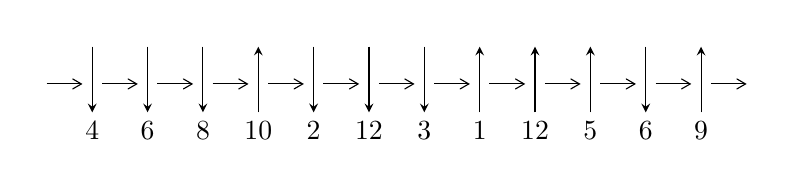
\begin{tikzpicture}[x=20pt, y=17pt]
	% nodes
	\node (C0) at (0, 0) {};
	\node (C1) at (1, 0) {};
	\node (C1U) at (1, +1) {};
	\node (C1D) at (1, -1) {4};

	\node (C2) at (2, 0) {};
	\node (C2U) at (2, +1) {};
	\node (C2D) at (2, -1) {6};

	\node (C3) at (3, 0) {};
	\node (C3U) at (3, +1) {};
	\node (C3D) at (3, -1) {8};

	\node (C4) at (4, 0) {};
	\node (C4U) at (4, +1) {};
	\node (C4D) at (4, -1) {10};

	\node (C5) at (5, 0) {};
	\node (C5U) at (5, +1) {};
	\node (C5D) at (5, -1) {2};

	\node (C6) at (6, 0) {};
	\node (C6U) at (6, +1) {};
	\node (C6D) at (6, -1) {12};

	\node (C7) at (7, 0) {};
	\node (C7U) at (7, +1) {};
	\node (C7D) at (7, -1) {3};

	\node (C8) at (8, 0) {};
	\node (C8U) at (8, +1) {};
	\node (C8D) at (8, -1) {1};

	\node (C9) at (9, 0) {};
	\node (C9U) at (9, +1) {};
	\node (C9D) at (9, -1) {12};

	\node (C10) at (10, 0) {};
	\node (C10U) at (10, +1) {};
	\node (C10D) at (10, -1) {5};

	\node (C11) at (11, 0) {};
	\node (C11U) at (11, +1) {};
	\node (C11D) at (11, -1) {6};

	\node (C12) at (12, 0) {};
	\node (C12U) at (12, +1) {};
	\node (C12D) at (12, -1) {9};
	\node (C13) at (13, 0) {};

	% arrows
	\draw[->,>={angle 60}]
	(C0) edge (C1) (C1) edge (C2) (C2) edge (C3) (C3) edge (C4) (C4) edge (C5) (C5) edge (C6) (C6) edge (C7) (C7) edge (C8) (C8) edge (C9) (C9) edge (C10) (C10) edge (C11) (C11) edge (C12) (C12) edge (C13) ;	\draw[->,>=stealth]
	(C1U) edge (C1D) (C2U) edge (C2D) (C3U) edge (C3D) (C4D) edge (C4U) (C5U) edge (C5D) (C6U) edge (C6D) (C7U) edge (C7D) (C8D) edge (C8U) (C9D) edge (C9U) (C10D) edge (C10U) (C11U) edge (C11D) (C12D) edge (C12U) ;
	\end{tikzpicture} \\
\hhline{~~} \\& 
\textbf{Solving Sequence} \\ \cline{2-2} 
 &
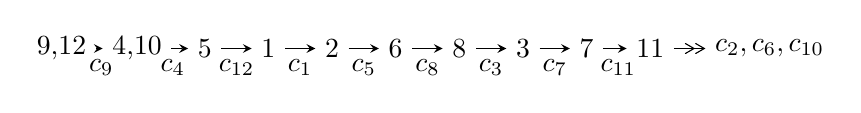
\begin{tikzpicture}[x=23pt, y=7pt]
	% node
	\node (A0) at (-1/8, 0) {9,12};
	\node (A1) at (17/16, 0) {4,10};
	\node (A2) at (17/8, 0) {5};
	\node (A3) at (25/8, 0) {1};
	\node (A4) at (33/8, 0) {2};
	\node (A5) at (41/8, 0) {6};
	\node (A6) at (49/8, 0) {8};
	\node (A7) at (57/8, 0) {3};
	\node (A8) at (65/8, 0) {7};
	\node (A9) at (73/8, 0) {11};
	\node (C1) at (1/2, -1) {$c_{9}$};
	\node (C2) at (13/8, -1) {$c_{4}$};
	\node (C3) at (21/8, -1) {$c_{12}$};
	\node (C4) at (29/8, -1) {$c_{1}$};
	\node (C5) at (37/8, -1) {$c_{5}$};
	\node (C6) at (45/8, -1) {$c_{8}$};
	\node (C7) at (53/8, -1) {$c_{3}$};
	\node (C8) at (61/8, -1) {$c_{7}$};
	\node (C9) at (69/8, -1) {$c_{11}$};
	\node (A10) at (11, 0) {$c_{2},c_{6},c_{10}$};

	% edge
	\draw[->,>=stealth]	
	(A0) edge (A1) (A1) edge (A2) (A2) edge (A3) (A3) edge (A4) (A4) edge (A5) (A5) edge (A6) (A6) edge (A7) (A7) edge (A8) (A8) edge (A9) ;
	\draw[->>,>={angle 60}]	
	(A9) edge (A10);
\end{tikzpicture} \\ 

\end{tabular} \\

\footnotetext{
The image of knot diagram is generated by the software ``\textbf{Draw programme}" developed by Andrew Bartholomew(\url{http://www.layer8.co.uk/maths/draw/index.htm\#Running-draw}), where we modified some parts for our purpose(\url{https://github.com/CATsTAILs/LinksPainter}).
}\phantom \\ \newline 
\centering \textbf{Ideals for irreducible components\footnotemark of $X_{\text{par}}$} 
 
\begin{align*}
I^u_{1}&=\langle 
744551414 u^{26}+8999949826 u^{25}+\cdots+22161981703 b-63305998448,\\
\phantom{I^u_{1}}&\phantom{= \langle  }51229810238 u^{26}-249479535086 u^{25}+\cdots+199457835327 a-467102435595,\\
\phantom{I^u_{1}}&\phantom{= \langle  }u^{27}-7 u^{26}+\cdots+69 u-9\rangle \\
I^u_{2}&=\langle 
4 u^{16} a+26 u^{16}+\cdots+14 a+91,\;3 u^{16} a+u^{16}+\cdots+2 a^2+8 a,\;u^{17}+3 u^{16}+\cdots+6 u+2\rangle \\
I^u_{3}&=\langle 
- u^{11}-4 u^{10}-12 u^9-25 u^8-41 u^7-54 u^6-58 u^5-51 u^4-36 u^3-20 u^2+b-8 u-2,\\
\phantom{I^u_{3}}&\phantom{= \langle  }2 u^{12}+3 u^{11}+8 u^{10}- u^9-16 u^8-58 u^7-96 u^6-131 u^5-128 u^4-105 u^3-60 u^2+5 a-28 u-4,\\
\phantom{I^u_{3}}&\phantom{= \langle  }u^{13}+4 u^{12}+14 u^{11}+32 u^{10}+62 u^9+96 u^8+127 u^7+142 u^6+136 u^5+110 u^4+75 u^3+41 u^2+18 u+5\rangle \\
I^u_{4}&=\langle 
a u+3 b-4 a+u-1,\;2 a^2+a u+2 a+4 u+3,\;u^2+2\rangle \\
\\
I^v_{1}&=\langle 
a,\;b- v+2,\;v^2-3 v+1\rangle \\
I^v_{2}&=\langle 
a,\;b+1,\;v-1\rangle \\
\end{align*}
\raggedright * 6 irreducible components of $\dim_{\mathbb{C}}=0$, with total 81 representations.\\
\footnotetext{All coefficients of polynomials are rational numbers. But the coefficients are sometimes approximated in decimal forms when there is not enough margin.}
\newpage
\renewcommand{\arraystretch}{1}
\centering \section*{I. $I^u_{1}= \langle 7.45\times10^{8} u^{26}+9.00\times10^{9} u^{25}+\cdots+2.22\times10^{10} b-6.33\times10^{10},\;5.12\times10^{10} u^{26}-2.49\times10^{11} u^{25}+\cdots+1.99\times10^{11} a-4.67\times10^{11},\;u^{27}-7 u^{26}+\cdots+69 u-9 \rangle$}
\flushleft \textbf{(i) Arc colorings}\\
\begin{tabular}{m{7pt} m{180pt} m{7pt} m{180pt} }
\flushright $a_{9}=$&$\begin{pmatrix}1\\0\end{pmatrix}$ \\
\flushright $a_{12}=$&$\begin{pmatrix}0\\u\end{pmatrix}$ \\
\flushright $a_{4}=$&$\begin{pmatrix}-0.256845 u^{26}+1.25079 u^{25}+\cdots-19.8801 u+2.34186\\-0.0335959 u^{26}-0.406099 u^{25}+\cdots-23.3945 u+2.85651\end{pmatrix}$ \\
\flushright $a_{10}=$&$\begin{pmatrix}1\\- u^2\end{pmatrix}$ \\
\flushright $a_{5}=$&$\begin{pmatrix}-0.427192 u^{26}+2.42462 u^{25}+\cdots-7.83439 u+0.274214\\-0.209462 u^{26}+0.793385 u^{25}+\cdots-23.1446 u+3.02389\end{pmatrix}$ \\
\flushright $a_{1}=$&$\begin{pmatrix}u\\u\end{pmatrix}$ \\
\flushright $a_{2}=$&$\begin{pmatrix}-0.373198 u^{26}+2.43639 u^{25}+\cdots+40.6429 u-5.57365\\0.0280075 u^{26}-0.274253 u^{25}+\cdots-15.2417 u+2.73067\end{pmatrix}$ \\
\flushright $a_{6}=$&$\begin{pmatrix}0.127411 u^{26}-0.794874 u^{25}+\cdots-16.3288 u+2.33469\\-0.220571 u^{26}+1.67833 u^{25}+\cdots+25.7235 u-4.23181\end{pmatrix}$ \\
\flushright $a_{8}=$&$\begin{pmatrix}u^2+1\\u^2\end{pmatrix}$ \\
\flushright $a_{3}=$&$\begin{pmatrix}0.229738 u^{26}-1.43782 u^{25}+\cdots-31.4394 u+3.80620\\0.547129 u^{26}-3.69315 u^{25}+\cdots-20.0642 u+2.31161\end{pmatrix}$ \\
\flushright $a_{7}=$&$\begin{pmatrix}0.127411 u^{26}-0.794874 u^{25}+\cdots-16.3288 u+2.33469\\-0.175997 u^{26}+1.30098 u^{25}+\cdots+20.1770 u-3.35878\end{pmatrix}$ \\
\flushright $a_{11}=$&$\begin{pmatrix}0.0573242 u^{26}-0.330383 u^{25}+\cdots-10.9429 u+1.67117\\-0.215260 u^{26}+1.35737 u^{25}+\cdots+7.85099 u-1.02783\end{pmatrix}$\\&\end{tabular}
\flushleft \textbf{(ii) Obstruction class $= -1$}\\~\\
\flushleft \textbf{(iii) Cusp Shapes $= -\frac{23743057753}{22161981703} u^{26}+\frac{150829290172}{22161981703} u^{25}+\cdots+\frac{2639501882667}{22161981703} u-\frac{630292627959}{22161981703}$}\\~\\
\newpage\renewcommand{\arraystretch}{1}
\flushleft \textbf{(iv) u-Polynomials at the component}\newline \\
\begin{tabular}{m{50pt}|m{274pt}}
Crossings & \hspace{64pt}u-Polynomials at each crossing \\
\hline $$\begin{aligned}c_{1},c_{3},c_{7}\end{aligned}$$&$\begin{aligned}
&u^{27}- u^{26}+\cdots+10 u-1
\end{aligned}$\\
\hline $$\begin{aligned}c_{2},c_{5}\end{aligned}$$&$\begin{aligned}
&u^{27}+11 u^{26}+\cdots-78 u-9
\end{aligned}$\\
\hline $$\begin{aligned}c_{4},c_{10}\end{aligned}$$&$\begin{aligned}
&u^{27}-2 u^{26}+\cdots+u+1
\end{aligned}$\\
\hline $$\begin{aligned}c_{6},c_{11}\end{aligned}$$&$\begin{aligned}
&u^{27}-2 u^{26}+\cdots+4 u+3
\end{aligned}$\\
\hline $$\begin{aligned}c_{8},c_{9},c_{12}\end{aligned}$$&$\begin{aligned}
&u^{27}+7 u^{26}+\cdots+69 u+9
\end{aligned}$\\
\hline
\end{tabular}\\~\\
\newpage\renewcommand{\arraystretch}{1}
\flushleft \textbf{(v) Riley Polynomials at the component}\newline \\
\begin{tabular}{m{50pt}|m{274pt}}
Crossings & \hspace{64pt}Riley Polynomials at each crossing \\
\hline $$\begin{aligned}c_{1},c_{3},c_{7}\end{aligned}$$&$\begin{aligned}
&y^{27}-25 y^{26}+\cdots+26 y-1
\end{aligned}$\\
\hline $$\begin{aligned}c_{2},c_{5}\end{aligned}$$&$\begin{aligned}
&y^{27}-7 y^{26}+\cdots-54 y-81
\end{aligned}$\\
\hline $$\begin{aligned}c_{4},c_{10}\end{aligned}$$&$\begin{aligned}
&y^{27}-22 y^{26}+\cdots+29 y-1
\end{aligned}$\\
\hline $$\begin{aligned}c_{6},c_{11}\end{aligned}$$&$\begin{aligned}
&y^{27}+22 y^{26}+\cdots+124 y-9
\end{aligned}$\\
\hline $$\begin{aligned}c_{8},c_{9},c_{12}\end{aligned}$$&$\begin{aligned}
&y^{27}+25 y^{26}+\cdots-1917 y-81
\end{aligned}$\\
\hline
\end{tabular}\\~\\
\newpage\flushleft \textbf{(vi) Complex Volumes and Cusp Shapes}
$$\begin{array}{c|c|c}  
\text{Solutions to }I^u_{1}& \I (\text{vol} + \sqrt{-1}CS) & \text{Cusp shape}\\
 \hline 
\begin{aligned}
u &= \phantom{-}0.953904 + 0.354754 I \\
a &= -1.047780 + 0.649531 I \\
b &= -0.214567 - 0.456094 I\end{aligned}
 & \phantom{-}4.79569 + 10.60650 I & -1.90397 - 7.23090 I \\ \hline\begin{aligned}
u &= \phantom{-}0.953904 - 0.354754 I \\
a &= -1.047780 - 0.649531 I \\
b &= -0.214567 + 0.456094 I\end{aligned}
 & \phantom{-}4.79569 - 10.60650 I & -1.90397 + 7.23090 I \\ \hline\begin{aligned}
u &= \phantom{-}0.933040 + 0.188802 I \\
a &= \phantom{-}1.160420 - 0.702560 I \\
b &= \phantom{-}0.051443 + 0.277504 I\end{aligned}
 & \phantom{-}4.62437 + 2.47514 I & -0.34993 - 2.26822 I \\ \hline\begin{aligned}
u &= \phantom{-}0.933040 - 0.188802 I \\
a &= \phantom{-}1.160420 + 0.702560 I \\
b &= \phantom{-}0.051443 - 0.277504 I\end{aligned}
 & \phantom{-}4.62437 - 2.47514 I & -0.34993 + 2.26822 I \\ \hline\begin{aligned}
u &= -0.478298 + 1.051980 I \\
a &= \phantom{-}0.189785 - 0.449325 I \\
b &= -0.036183 - 0.475615 I\end{aligned}
 & -0.42491 - 2.93654 I & \phantom{-}4.22853 + 4.23030 I \\ \hline\begin{aligned}
u &= -0.478298 - 1.051980 I \\
a &= \phantom{-}0.189785 + 0.449325 I \\
b &= -0.036183 + 0.475615 I\end{aligned}
 & -0.42491 + 2.93654 I & \phantom{-}4.22853 - 4.23030 I \\ \hline\begin{aligned}
u &= -0.645899 + 0.517518 I \\
a &= \phantom{-}0.674135 + 0.117637 I \\
b &= \phantom{-}0.442860 - 0.100682 I\end{aligned}
 & \phantom{-}1.19510 - 1.40624 I & \phantom{-}0.86573 + 1.18666 I \\ \hline\begin{aligned}
u &= -0.645899 - 0.517518 I \\
a &= \phantom{-}0.674135 - 0.117637 I \\
b &= \phantom{-}0.442860 + 0.100682 I\end{aligned}
 & \phantom{-}1.19510 + 1.40624 I & \phantom{-}0.86573 - 1.18666 I \\ \hline\begin{aligned}
u &= \phantom{-}0.721039 + 0.972434 I \\
a &= -0.052879 - 0.387807 I \\
b &= \phantom{-}0.717442 - 0.773808 I\end{aligned}
 & \phantom{-}2.98852 - 4.83503 I & -4.24483 + 4.00030 I \\ \hline\begin{aligned}
u &= \phantom{-}0.721039 - 0.972434 I \\
a &= -0.052879 + 0.387807 I \\
b &= \phantom{-}0.717442 + 0.773808 I\end{aligned}
 & \phantom{-}2.98852 + 4.83503 I & -4.24483 - 4.00030 I\\
 \hline 
 \end{array}$$\newpage$$\begin{array}{c|c|c}  
\text{Solutions to }I^u_{1}& \I (\text{vol} + \sqrt{-1}CS) & \text{Cusp shape}\\
 \hline 
\begin{aligned}
u &= \phantom{-}0.553346 + 1.170330 I \\
a &= -0.353880 + 0.426742 I \\
b &= -1.03955 + 0.97978 I\end{aligned}
 & \phantom{-}1.66563 + 2.80958 I & -3.84805 - 1.74078 I \\ \hline\begin{aligned}
u &= \phantom{-}0.553346 - 1.170330 I \\
a &= -0.353880 - 0.426742 I \\
b &= -1.03955 - 0.97978 I\end{aligned}
 & \phantom{-}1.66563 - 2.80958 I & -3.84805 + 1.74078 I \\ \hline\begin{aligned}
u &= \phantom{-}0.654565\phantom{ +0.000000I} \\
a &= -1.70509\phantom{ +0.000000I} \\
b &= \phantom{-}0.498180\phantom{ +0.000000I}\end{aligned}
 & -7.54449\phantom{ +0.000000I} & -20.1420\phantom{ +0.000000I} \\ \hline\begin{aligned}
u &= \phantom{-}0.025050 + 1.359590 I \\
a &= -0.84354 + 1.28631 I \\
b &= -0.46291 + 2.19675 I\end{aligned}
 & -6.22130 + 0.13227 I & -6.04494 + 0.29033 I \\ \hline\begin{aligned}
u &= \phantom{-}0.025050 - 1.359590 I \\
a &= -0.84354 - 1.28631 I \\
b &= -0.46291 - 2.19675 I\end{aligned}
 & -6.22130 - 0.13227 I & -6.04494 - 0.29033 I \\ \hline\begin{aligned}
u &= \phantom{-}0.255910 + 1.345710 I \\
a &= \phantom{-}0.724542 - 1.206850 I \\
b &= \phantom{-}0.67761 - 2.38128 I\end{aligned}
 & -11.88730 + 3.29707 I & -9.75000 + 3.82687 I \\ \hline\begin{aligned}
u &= \phantom{-}0.255910 - 1.345710 I \\
a &= \phantom{-}0.724542 + 1.206850 I \\
b &= \phantom{-}0.67761 + 2.38128 I\end{aligned}
 & -11.88730 - 3.29707 I & -9.75000 - 3.82687 I \\ \hline\begin{aligned}
u &= \phantom{-}0.00342 + 1.44547 I \\
a &= -0.51617 + 1.50351 I \\
b &= -0.02636 + 2.23591 I\end{aligned}
 & -6.76916 + 0.50453 I & -6.09785 - 2.87578 I \\ \hline\begin{aligned}
u &= \phantom{-}0.00342 - 1.44547 I \\
a &= -0.51617 - 1.50351 I \\
b &= -0.02636 - 2.23591 I\end{aligned}
 & -6.76916 - 0.50453 I & -6.09785 + 2.87578 I \\ \hline\begin{aligned}
u &= \phantom{-}0.38425 + 1.40937 I \\
a &= -0.04227 + 1.48372 I \\
b &= \phantom{-}0.22763 + 2.62497 I\end{aligned}
 & -0.46126 + 7.18382 I & -3.58916 - 3.85062 I\\
 \hline 
 \end{array}$$\newpage$$\begin{array}{c|c|c}  
\text{Solutions to }I^u_{1}& \I (\text{vol} + \sqrt{-1}CS) & \text{Cusp shape}\\
 \hline 
\begin{aligned}
u &= \phantom{-}0.38425 - 1.40937 I \\
a &= -0.04227 - 1.48372 I \\
b &= \phantom{-}0.22763 - 2.62497 I\end{aligned}
 & -0.46126 - 7.18382 I & -3.58916 + 3.85062 I \\ \hline\begin{aligned}
u &= \phantom{-}0.37205 + 1.48920 I \\
a &= -0.05733 - 1.69219 I \\
b &= -0.38069 - 2.77325 I\end{aligned}
 & -1.1155 + 15.3839 I & -5.17512 - 7.69230 I \\ \hline\begin{aligned}
u &= \phantom{-}0.37205 - 1.48920 I \\
a &= -0.05733 + 1.69219 I \\
b &= -0.38069 + 2.77325 I\end{aligned}
 & -1.1155 - 15.3839 I & -5.17512 + 7.69230 I \\ \hline\begin{aligned}
u &= \phantom{-}0.01460 + 1.56688 I \\
a &= \phantom{-}0.523915 - 1.145590 I \\
b &= \phantom{-}0.30647 - 1.70007 I\end{aligned}
 & -6.50814 - 3.09204 I & -6.77423 + 4.55905 I \\ \hline\begin{aligned}
u &= \phantom{-}0.01460 - 1.56688 I \\
a &= \phantom{-}0.523915 + 1.145590 I \\
b &= \phantom{-}0.30647 + 1.70007 I\end{aligned}
 & -6.50814 + 3.09204 I & -6.77423 - 4.55905 I \\ \hline\begin{aligned}
u &= \phantom{-}0.080303 + 0.257685 I \\
a &= -0.67306 - 2.09112 I \\
b &= -0.512295 + 0.381584 I\end{aligned}
 & -1.138560 + 0.334603 I & -9.24522 - 1.52255 I \\ \hline\begin{aligned}
u &= \phantom{-}0.080303 - 0.257685 I \\
a &= -0.67306 + 2.09112 I \\
b &= -0.512295 - 0.381584 I\end{aligned}
 & -1.138560 - 0.334603 I & -9.24522 + 1.52255 I\\
 \hline 
 \end{array}$$\newpage\newpage\renewcommand{\arraystretch}{1}
\centering \section*{II. $I^u_{2}= \langle 4 u^{16} a+26 u^{16}+\cdots+14 a+91,\;3 u^{16} a+u^{16}+\cdots+2 a^2+8 a,\;u^{17}+3 u^{16}+\cdots+6 u+2 \rangle$}
\flushleft \textbf{(i) Arc colorings}\\
\begin{tabular}{m{7pt} m{180pt} m{7pt} m{180pt} }
\flushright $a_{9}=$&$\begin{pmatrix}1\\0\end{pmatrix}$ \\
\flushright $a_{12}=$&$\begin{pmatrix}0\\u\end{pmatrix}$ \\
\flushright $a_{4}=$&$\begin{pmatrix}a\\-0.108108 a u^{16}-0.702703 u^{16}+\cdots-0.378378 a-2.45946\end{pmatrix}$ \\
\flushright $a_{10}=$&$\begin{pmatrix}1\\- u^2\end{pmatrix}$ \\
\flushright $a_{5}=$&$\begin{pmatrix}-0.108108 a u^{16}-0.702703 u^{16}+\cdots+0.621622 a-2.45946\\-0.297297 a u^{16}-1.43243 u^{16}+\cdots-0.540541 a-2.51351\end{pmatrix}$ \\
\flushright $a_{1}=$&$\begin{pmatrix}u\\u\end{pmatrix}$ \\
\flushright $a_{2}=$&$\begin{pmatrix}0.0270270 a u^{16}+0.175676 u^{16}+\cdots-2.40541 a-1.13514\\0.729730 a u^{16}+0.243243 u^{16}+\cdots+0.0540541 a-1.64865\end{pmatrix}$ \\
\flushright $a_{6}=$&$\begin{pmatrix}-0.243243 a u^{16}-0.581081 u^{16}+\cdots-1.35135 a-2.78378\\0.0540541 a u^{16}-0.648649 u^{16}+\cdots-0.810811 a-2.27027\end{pmatrix}$ \\
\flushright $a_{8}=$&$\begin{pmatrix}u^2+1\\u^2\end{pmatrix}$ \\
\flushright $a_{3}=$&$\begin{pmatrix}0.189189 a u^{16}-0.270270 u^{16}+\cdots+1.16216 a-2.94595\\- u^{16}-3 u^{15}+\cdots-5 u-3\end{pmatrix}$ \\
\flushright $a_{7}=$&$\begin{pmatrix}-0.243243 a u^{16}-0.581081 u^{16}+\cdots-1.35135 a-2.78378\\-0.270270 a u^{16}-0.756757 u^{16}+\cdots+0.0540541 a-2.64865\end{pmatrix}$ \\
\flushright $a_{11}=$&$\begin{pmatrix}0.0810811 a u^{16}-0.472973 u^{16}+\cdots-0.216216 a-2.40541\\-0.324324 a u^{16}-0.108108 u^{16}+\cdots-1.13514 a-2.37838\end{pmatrix}$\\&\end{tabular}
\flushleft \textbf{(ii) Obstruction class $= -1$}\\~\\
\flushleft \textbf{(iii) Cusp Shapes $= 3 u^{16}+9 u^{15}+35 u^{14}+74 u^{13}+150 u^{12}+231 u^{11}+301 u^{10}+324 u^9+266 u^8+150 u^7+22 u^6-76 u^5-96 u^4-61 u^3-15 u^2+12 u+14$}\\~\\
\newpage\renewcommand{\arraystretch}{1}
\flushleft \textbf{(iv) u-Polynomials at the component}\newline \\
\begin{tabular}{m{50pt}|m{274pt}}
Crossings & \hspace{64pt}u-Polynomials at each crossing \\
\hline $$\begin{aligned}c_{1},c_{3},c_{7}\end{aligned}$$&$\begin{aligned}
&u^{34}+2 u^{33}+\cdots+51 u-23
\end{aligned}$\\
\hline $$\begin{aligned}c_{2},c_{5}\end{aligned}$$&$\begin{aligned}
&(u^{17}-4 u^{16}+\cdots-4 u+1)^{2}
\end{aligned}$\\
\hline $$\begin{aligned}c_{4},c_{10}\end{aligned}$$&$\begin{aligned}
&u^{34}-15 u^{32}+\cdots-37 u+61
\end{aligned}$\\
\hline $$\begin{aligned}c_{6},c_{11}\end{aligned}$$&$\begin{aligned}
&u^{34}+3 u^{33}+\cdots-682 u-121
\end{aligned}$\\
\hline $$\begin{aligned}c_{8},c_{9},c_{12}\end{aligned}$$&$\begin{aligned}
&(u^{17}-3 u^{16}+\cdots+6 u-2)^{2}
\end{aligned}$\\
\hline
\end{tabular}\\~\\
\newpage\renewcommand{\arraystretch}{1}
\flushleft \textbf{(v) Riley Polynomials at the component}\newline \\
\begin{tabular}{m{50pt}|m{274pt}}
Crossings & \hspace{64pt}Riley Polynomials at each crossing \\
\hline $$\begin{aligned}c_{1},c_{3},c_{7}\end{aligned}$$&$\begin{aligned}
&y^{34}-6 y^{33}+\cdots-7293 y+529
\end{aligned}$\\
\hline $$\begin{aligned}c_{2},c_{5}\end{aligned}$$&$\begin{aligned}
&(y^{17}-2 y^{16}+\cdots-4 y-1)^{2}
\end{aligned}$\\
\hline $$\begin{aligned}c_{4},c_{10}\end{aligned}$$&$\begin{aligned}
&y^{34}-30 y^{33}+\cdots-156553 y+3721
\end{aligned}$\\
\hline $$\begin{aligned}c_{6},c_{11}\end{aligned}$$&$\begin{aligned}
&y^{34}+29 y^{33}+\cdots+783838 y+14641
\end{aligned}$\\
\hline $$\begin{aligned}c_{8},c_{9},c_{12}\end{aligned}$$&$\begin{aligned}
&(y^{17}+17 y^{16}+\cdots+52 y-4)^{2}
\end{aligned}$\\
\hline
\end{tabular}\\~\\
\newpage\flushleft \textbf{(vi) Complex Volumes and Cusp Shapes}
$$\begin{array}{c|c|c}  
\text{Solutions to }I^u_{2}& \I (\text{vol} + \sqrt{-1}CS) & \text{Cusp shape}\\
 \hline 
\begin{aligned}
u &= -0.700839 + 0.661242 I \\
a &= -0.142439 - 0.723173 I \\
b &= -0.131868 + 0.225388 I\end{aligned}
 & \phantom{-}0.33195 - 3.39163 I & -2.33298 + 11.95319 I \\ \hline\begin{aligned}
u &= -0.700839 + 0.661242 I \\
a &= \phantom{-}0.440456 - 0.231356 I \\
b &= \phantom{-}0.065889 - 0.965375 I\end{aligned}
 & \phantom{-}0.33195 - 3.39163 I & -2.33298 + 11.95319 I \\ \hline\begin{aligned}
u &= -0.700839 - 0.661242 I \\
a &= -0.142439 + 0.723173 I \\
b &= -0.131868 - 0.225388 I\end{aligned}
 & \phantom{-}0.33195 + 3.39163 I & -2.33298 - 11.95319 I \\ \hline\begin{aligned}
u &= -0.700839 - 0.661242 I \\
a &= \phantom{-}0.440456 + 0.231356 I \\
b &= \phantom{-}0.065889 + 0.965375 I\end{aligned}
 & \phantom{-}0.33195 + 3.39163 I & -2.33298 - 11.95319 I \\ \hline\begin{aligned}
u &= -0.826403 + 0.349944 I \\
a &= \phantom{-}1.075520 + 0.373580 I \\
b &= \phantom{-}0.414461 - 0.303701 I\end{aligned}
 & \phantom{-}1.33448 - 1.66721 I & \phantom{-}5.61922 + 1.37527 I \\ \hline\begin{aligned}
u &= -0.826403 + 0.349944 I \\
a &= \phantom{-}0.164500 - 0.258544 I \\
b &= \phantom{-}0.390587 + 0.201368 I\end{aligned}
 & \phantom{-}1.33448 - 1.66721 I & \phantom{-}5.61922 + 1.37527 I \\ \hline\begin{aligned}
u &= -0.826403 - 0.349944 I \\
a &= \phantom{-}1.075520 - 0.373580 I \\
b &= \phantom{-}0.414461 + 0.303701 I\end{aligned}
 & \phantom{-}1.33448 + 1.66721 I & \phantom{-}5.61922 - 1.37527 I \\ \hline\begin{aligned}
u &= -0.826403 - 0.349944 I \\
a &= \phantom{-}0.164500 + 0.258544 I \\
b &= \phantom{-}0.390587 - 0.201368 I\end{aligned}
 & \phantom{-}1.33448 + 1.66721 I & \phantom{-}5.61922 - 1.37527 I \\ \hline\begin{aligned}
u &= \phantom{-}0.177657 + 1.249920 I \\
a &= \phantom{-}0.369639 + 0.260996 I \\
b &= -0.914870 + 0.498586 I\end{aligned}
 & \phantom{-}3.03460 - 1.26688 I & -4.55357 - 0.56113 I \\ \hline\begin{aligned}
u &= \phantom{-}0.177657 + 1.249920 I \\
a &= -1.00148 - 1.87787 I \\
b &= -1.23762 - 2.66817 I\end{aligned}
 & \phantom{-}3.03460 - 1.26688 I & -4.55357 - 0.56113 I\\
 \hline 
 \end{array}$$\newpage$$\begin{array}{c|c|c}  
\text{Solutions to }I^u_{2}& \I (\text{vol} + \sqrt{-1}CS) & \text{Cusp shape}\\
 \hline 
\begin{aligned}
u &= \phantom{-}0.177657 - 1.249920 I \\
a &= \phantom{-}0.369639 - 0.260996 I \\
b &= -0.914870 - 0.498586 I\end{aligned}
 & \phantom{-}3.03460 + 1.26688 I & -4.55357 + 0.56113 I \\ \hline\begin{aligned}
u &= \phantom{-}0.177657 - 1.249920 I \\
a &= -1.00148 + 1.87787 I \\
b &= -1.23762 + 2.66817 I\end{aligned}
 & \phantom{-}3.03460 + 1.26688 I & -4.55357 + 0.56113 I \\ \hline\begin{aligned}
u &= \phantom{-}0.177527 + 1.341090 I \\
a &= \phantom{-}0.078205 - 0.428055 I \\
b &= \phantom{-}1.44700 - 0.65077 I\end{aligned}
 & \phantom{-}2.28668 + 6.31784 I & -5.66125 - 5.46008 I \\ \hline\begin{aligned}
u &= \phantom{-}0.177527 + 1.341090 I \\
a &= \phantom{-}1.01930 + 2.21437 I \\
b &= \phantom{-}1.22445 + 2.88700 I\end{aligned}
 & \phantom{-}2.28668 + 6.31784 I & -5.66125 - 5.46008 I \\ \hline\begin{aligned}
u &= \phantom{-}0.177527 - 1.341090 I \\
a &= \phantom{-}0.078205 + 0.428055 I \\
b &= \phantom{-}1.44700 + 0.65077 I\end{aligned}
 & \phantom{-}2.28668 - 6.31784 I & -5.66125 + 5.46008 I \\ \hline\begin{aligned}
u &= \phantom{-}0.177527 - 1.341090 I \\
a &= \phantom{-}1.01930 - 2.21437 I \\
b &= \phantom{-}1.22445 - 2.88700 I\end{aligned}
 & \phantom{-}2.28668 - 6.31784 I & -5.66125 + 5.46008 I \\ \hline\begin{aligned}
u &= -0.132324 + 1.358820 I \\
a &= -1.303170 - 0.221965 I \\
b &= -0.815188 - 0.630532 I\end{aligned}
 & -7.55907 - 1.70238 I & -7.27343 + 3.59367 I \\ \hline\begin{aligned}
u &= -0.132324 + 1.358820 I \\
a &= \phantom{-}0.07650 + 1.87317 I \\
b &= \phantom{-}0.16530 + 3.22936 I\end{aligned}
 & -7.55907 - 1.70238 I & -7.27343 + 3.59367 I \\ \hline\begin{aligned}
u &= -0.132324 - 1.358820 I \\
a &= -1.303170 + 0.221965 I \\
b &= -0.815188 + 0.630532 I\end{aligned}
 & -7.55907 + 1.70238 I & -7.27343 - 3.59367 I \\ \hline\begin{aligned}
u &= -0.132324 - 1.358820 I \\
a &= \phantom{-}0.07650 - 1.87317 I \\
b &= \phantom{-}0.16530 - 3.22936 I\end{aligned}
 & -7.55907 + 1.70238 I & -7.27343 - 3.59367 I\\
 \hline 
 \end{array}$$\newpage$$\begin{array}{c|c|c}  
\text{Solutions to }I^u_{2}& \I (\text{vol} + \sqrt{-1}CS) & \text{Cusp shape}\\
 \hline 
\begin{aligned}
u &= -0.31944 + 1.42784 I \\
a &= \phantom{-}0.286545 + 0.562334 I \\
b &= -0.176253 + 1.206940 I\end{aligned}
 & -4.28217 - 5.80165 I & -2.59768 + 6.29733 I \\ \hline\begin{aligned}
u &= -0.31944 + 1.42784 I \\
a &= \phantom{-}0.13016 - 1.68353 I \\
b &= \phantom{-}0.18891 - 2.61278 I\end{aligned}
 & -4.28217 - 5.80165 I & -2.59768 + 6.29733 I \\ \hline\begin{aligned}
u &= -0.31944 - 1.42784 I \\
a &= \phantom{-}0.286545 - 0.562334 I \\
b &= -0.176253 - 1.206940 I\end{aligned}
 & -4.28217 + 5.80165 I & -2.59768 - 6.29733 I \\ \hline\begin{aligned}
u &= -0.31944 - 1.42784 I \\
a &= \phantom{-}0.13016 + 1.68353 I \\
b &= \phantom{-}0.18891 + 2.61278 I\end{aligned}
 & -4.28217 + 5.80165 I & -2.59768 - 6.29733 I \\ \hline\begin{aligned}
u &= \phantom{-}0.523959 + 0.054315 I \\
a &= \phantom{-}1.90743 - 1.36602 I \\
b &= \phantom{-}0.986066 + 0.652053 I\end{aligned}
 & \phantom{-}6.73749 + 3.81968 I & \phantom{-}1.95892 - 3.35628 I \\ \hline\begin{aligned}
u &= \phantom{-}0.523959 + 0.054315 I \\
a &= -2.25261 - 1.67330 I \\
b &= -0.855397 + 0.372276 I\end{aligned}
 & \phantom{-}6.73749 + 3.81968 I & \phantom{-}1.95892 - 3.35628 I \\ \hline\begin{aligned}
u &= \phantom{-}0.523959 - 0.054315 I \\
a &= \phantom{-}1.90743 + 1.36602 I \\
b &= \phantom{-}0.986066 - 0.652053 I\end{aligned}
 & \phantom{-}6.73749 - 3.81968 I & \phantom{-}1.95892 + 3.35628 I \\ \hline\begin{aligned}
u &= \phantom{-}0.523959 - 0.054315 I \\
a &= -2.25261 + 1.67330 I \\
b &= -0.855397 - 0.372276 I\end{aligned}
 & \phantom{-}6.73749 - 3.81968 I & \phantom{-}1.95892 + 3.35628 I \\ \hline\begin{aligned}
u &= -0.23365 + 1.55973 I \\
a &= -0.266571 + 1.360880 I \\
b &= -0.73106 + 2.22334 I\end{aligned}
 & -6.94898 - 6.84809 I & -12.0162 + 9.7020 I \\ \hline\begin{aligned}
u &= -0.23365 + 1.55973 I \\
a &= -0.43195 - 1.69334 I \\
b &= -0.20577 - 2.36976 I\end{aligned}
 & -6.94898 - 6.84809 I & -12.0162 + 9.7020 I\\
 \hline 
 \end{array}$$\newpage$$\begin{array}{c|c|c}  
\text{Solutions to }I^u_{2}& \I (\text{vol} + \sqrt{-1}CS) & \text{Cusp shape}\\
 \hline 
\begin{aligned}
u &= -0.23365 - 1.55973 I \\
a &= -0.266571 - 1.360880 I \\
b &= -0.73106 - 2.22334 I\end{aligned}
 & -6.94898 + 6.84809 I & -12.0162 - 9.7020 I \\ \hline\begin{aligned}
u &= -0.23365 - 1.55973 I \\
a &= -0.43195 + 1.69334 I \\
b &= -0.20577 + 2.36976 I\end{aligned}
 & -6.94898 + 6.84809 I & -12.0162 - 9.7020 I \\ \hline\begin{aligned}
u &= -0.332972\phantom{ +0.000000I} \\
a &= -0.266953\phantom{ +0.000000I} \\
b &= -1.49504\phantom{ +0.000000I}\end{aligned}
 & -3.02943\phantom{ +0.000000I} & \phantom{-}9.71400\phantom{ +0.000000I} \\ \hline\begin{aligned}
u &= -0.332972\phantom{ +0.000000I} \\
a &= -5.03314\phantom{ +0.000000I} \\
b &= -0.134225\phantom{ +0.000000I}\end{aligned}
 & -3.02943\phantom{ +0.000000I} & \phantom{-}9.71400\phantom{ +0.000000I}\\
 \hline 
 \end{array}$$\newpage\newpage\renewcommand{\arraystretch}{1}
\centering \section*{III. $I^u_{3}= \langle - u^{11}-4 u^{10}+\cdots+b-2,\;2 u^{12}+3 u^{11}+\cdots+5 a-4,\;u^{13}+4 u^{12}+\cdots+18 u+5 \rangle$}
\flushleft \textbf{(i) Arc colorings}\\
\begin{tabular}{m{7pt} m{180pt} m{7pt} m{180pt} }
\flushright $a_{9}=$&$\begin{pmatrix}1\\0\end{pmatrix}$ \\
\flushright $a_{12}=$&$\begin{pmatrix}0\\u\end{pmatrix}$ \\
\flushright $a_{4}=$&$\begin{pmatrix}-\frac{2}{5} u^{12}-\frac{3}{5} u^{11}+\cdots+\frac{28}{5} u+\frac{4}{5}\\u^{11}+4 u^{10}+\cdots+8 u+2\end{pmatrix}$ \\
\flushright $a_{10}=$&$\begin{pmatrix}1\\- u^2\end{pmatrix}$ \\
\flushright $a_{5}=$&$\begin{pmatrix}-\frac{2}{5} u^{12}-\frac{3}{5} u^{11}+\cdots-\frac{12}{5} u-\frac{11}{5}\\u^{11}+5 u^{10}+\cdots+8 u+2\end{pmatrix}$ \\
\flushright $a_{1}=$&$\begin{pmatrix}u\\u\end{pmatrix}$ \\
\flushright $a_{2}=$&$\begin{pmatrix}\frac{4}{5} u^{12}+\frac{11}{5} u^{11}+\cdots+\frac{14}{5} u+\frac{7}{5}\\- u^{11}-4 u^{10}+\cdots-12 u-4\end{pmatrix}$ \\
\flushright $a_{6}=$&$\begin{pmatrix}-\frac{1}{5} u^{12}-\frac{4}{5} u^{11}+\cdots-\frac{36}{5} u-\frac{8}{5}\\- u^{12}-4 u^{11}+\cdots-14 u-4\end{pmatrix}$ \\
\flushright $a_{8}=$&$\begin{pmatrix}u^2+1\\u^2\end{pmatrix}$ \\
\flushright $a_{3}=$&$\begin{pmatrix}\frac{3}{5} u^{12}+\frac{12}{5} u^{11}+\cdots+\frac{58}{5} u+\frac{14}{5}\\u^{12}+4 u^{11}+\cdots+8 u+2\end{pmatrix}$ \\
\flushright $a_{7}=$&$\begin{pmatrix}-\frac{1}{5} u^{12}-\frac{4}{5} u^{11}+\cdots-\frac{36}{5} u-\frac{8}{5}\\- u^{12}-4 u^{11}+\cdots-13 u-4\end{pmatrix}$ \\
\flushright $a_{11}=$&$\begin{pmatrix}-\frac{1}{5} u^{12}-\frac{4}{5} u^{11}+\cdots-\frac{11}{5} u+\frac{2}{5}\\- u^7-2 u^6-4 u^5-4 u^4-2 u^3+2 u+1\end{pmatrix}$\\&\end{tabular}
\flushleft \textbf{(ii) Obstruction class $= 1$}\\~\\
\flushleft \textbf{(iii) Cusp Shapes $= 4 u^{12}+12 u^{11}+41 u^{10}+76 u^9+135 u^8+174 u^7+202 u^6+192 u^5+158 u^4+106 u^3+63 u^2+27 u+8$}\\~\\
\newpage\renewcommand{\arraystretch}{1}
\flushleft \textbf{(iv) u-Polynomials at the component}\newline \\
\begin{tabular}{m{50pt}|m{274pt}}
Crossings & \hspace{64pt}u-Polynomials at each crossing \\
\hline $$\begin{aligned}c_{1},c_{3}\end{aligned}$$&$\begin{aligned}
&u^{13}-3 u^{11}+\cdots-5 u+1
\end{aligned}$\\
\hline $$\begin{aligned}c_{2}\end{aligned}$$&$\begin{aligned}
&u^{13}+8 u^{12}+\cdots+3 u+1
\end{aligned}$\\
\hline $$\begin{aligned}c_{4}\end{aligned}$$&$\begin{aligned}
&u^{13}- u^{12}+\cdots+2 u-1
\end{aligned}$\\
\hline $$\begin{aligned}c_{5}\end{aligned}$$&$\begin{aligned}
&u^{13}-8 u^{12}+\cdots+3 u-1
\end{aligned}$\\
\hline $$\begin{aligned}c_{6}\end{aligned}$$&$\begin{aligned}
&u^{13}- u^{12}+\cdots- u+1
\end{aligned}$\\
\hline $$\begin{aligned}c_{7}\end{aligned}$$&$\begin{aligned}
&u^{13}-3 u^{11}+\cdots-5 u-1
\end{aligned}$\\
\hline $$\begin{aligned}c_{8},c_{9}\end{aligned}$$&$\begin{aligned}
&u^{13}+4 u^{12}+\cdots+18 u+5
\end{aligned}$\\
\hline $$\begin{aligned}c_{10}\end{aligned}$$&$\begin{aligned}
&u^{13}+u^{12}+\cdots+2 u+1
\end{aligned}$\\
\hline $$\begin{aligned}c_{11}\end{aligned}$$&$\begin{aligned}
&u^{13}+u^{12}+\cdots- u-1
\end{aligned}$\\
\hline $$\begin{aligned}c_{12}\end{aligned}$$&$\begin{aligned}
&u^{13}-4 u^{12}+\cdots+18 u-5
\end{aligned}$\\
\hline
\end{tabular}\\~\\
\newpage\renewcommand{\arraystretch}{1}
\flushleft \textbf{(v) Riley Polynomials at the component}\newline \\
\begin{tabular}{m{50pt}|m{274pt}}
Crossings & \hspace{64pt}Riley Polynomials at each crossing \\
\hline $$\begin{aligned}c_{1},c_{3},c_{7}\end{aligned}$$&$\begin{aligned}
&y^{13}-6 y^{12}+\cdots+5 y-1
\end{aligned}$\\
\hline $$\begin{aligned}c_{2},c_{5}\end{aligned}$$&$\begin{aligned}
&y^{13}-8 y^{12}+\cdots-7 y-1
\end{aligned}$\\
\hline $$\begin{aligned}c_{4},c_{10}\end{aligned}$$&$\begin{aligned}
&y^{13}-7 y^{12}+\cdots+8 y-1
\end{aligned}$\\
\hline $$\begin{aligned}c_{6},c_{11}\end{aligned}$$&$\begin{aligned}
&y^{13}+13 y^{12}+\cdots+3 y-1
\end{aligned}$\\
\hline $$\begin{aligned}c_{8},c_{9},c_{12}\end{aligned}$$&$\begin{aligned}
&y^{13}+12 y^{12}+\cdots-86 y-25
\end{aligned}$\\
\hline
\end{tabular}\\~\\
\newpage\flushleft \textbf{(vi) Complex Volumes and Cusp Shapes}
$$\begin{array}{c|c|c}  
\text{Solutions to }I^u_{3}& \I (\text{vol} + \sqrt{-1}CS) & \text{Cusp shape}\\
 \hline 
\begin{aligned}
u &= -0.870086 + 0.472668 I \\
a &= \phantom{-}0.562228 + 0.256963 I \\
b &= \phantom{-}0.058997 - 0.395621 I\end{aligned}
 & \phantom{-}0.72518 - 2.27010 I & -3.32570 + 6.32204 I \\ \hline\begin{aligned}
u &= -0.870086 - 0.472668 I \\
a &= \phantom{-}0.562228 - 0.256963 I \\
b &= \phantom{-}0.058997 + 0.395621 I\end{aligned}
 & \phantom{-}0.72518 + 2.27010 I & -3.32570 - 6.32204 I \\ \hline\begin{aligned}
u &= \phantom{-}0.188480 + 1.095940 I \\
a &= \phantom{-}0.015018 + 1.370830 I \\
b &= -0.89332 + 1.36698 I\end{aligned}
 & \phantom{-}3.78493 + 4.55783 I & -2.53815 - 3.04000 I \\ \hline\begin{aligned}
u &= \phantom{-}0.188480 - 1.095940 I \\
a &= \phantom{-}0.015018 - 1.370830 I \\
b &= -0.89332 - 1.36698 I\end{aligned}
 & \phantom{-}3.78493 - 4.55783 I & -2.53815 + 3.04000 I \\ \hline\begin{aligned}
u &= \phantom{-}0.201492 + 0.859165 I \\
a &= -0.371227 - 1.303860 I \\
b &= \phantom{-}0.659133 - 1.181080 I\end{aligned}
 & \phantom{-}4.68144 - 3.00710 I & -1.90498 + 2.28394 I \\ \hline\begin{aligned}
u &= \phantom{-}0.201492 - 0.859165 I \\
a &= -0.371227 + 1.303860 I \\
b &= \phantom{-}0.659133 + 1.181080 I\end{aligned}
 & \phantom{-}4.68144 + 3.00710 I & -1.90498 - 2.28394 I \\ \hline\begin{aligned}
u &= -0.544012 + 1.038490 I \\
a &= -0.075020 - 0.146685 I \\
b &= -0.404699 - 0.503620 I\end{aligned}
 & -0.91635 - 2.84840 I & -12.09656 + 1.44482 I \\ \hline\begin{aligned}
u &= -0.544012 - 1.038490 I \\
a &= -0.075020 + 0.146685 I \\
b &= -0.404699 + 0.503620 I\end{aligned}
 & -0.91635 + 2.84840 I & -12.09656 - 1.44482 I \\ \hline\begin{aligned}
u &= -0.758405\phantom{ +0.000000I} \\
a &= -1.58340\phantom{ +0.000000I} \\
b &= \phantom{-}0.355204\phantom{ +0.000000I}\end{aligned}
 & -7.22673\phantom{ +0.000000I} & \phantom{-}5.56510\phantom{ +0.000000I} \\ \hline\begin{aligned}
u &= -0.32313 + 1.38540 I \\
a &= \phantom{-}0.602248 + 1.222900 I \\
b &= \phantom{-}0.65830 + 2.32161 I\end{aligned}
 & -11.73130 - 3.93288 I & -6.70847 + 7.41271 I\\
 \hline 
 \end{array}$$\newpage$$\begin{array}{c|c|c}  
\text{Solutions to }I^u_{3}& \I (\text{vol} + \sqrt{-1}CS) & \text{Cusp shape}\\
 \hline 
\begin{aligned}
u &= -0.32313 - 1.38540 I \\
a &= \phantom{-}0.602248 - 1.222900 I \\
b &= \phantom{-}0.65830 - 2.32161 I\end{aligned}
 & -11.73130 + 3.93288 I & -6.70847 - 7.41271 I \\ \hline\begin{aligned}
u &= -0.27355 + 1.56061 I \\
a &= -0.041547 - 1.376770 I \\
b &= \phantom{-}0.24399 - 2.09573 I\end{aligned}
 & -6.09001 - 6.43621 I & -3.20871 + 5.54804 I \\ \hline\begin{aligned}
u &= -0.27355 - 1.56061 I \\
a &= -0.041547 + 1.376770 I \\
b &= \phantom{-}0.24399 + 2.09573 I\end{aligned}
 & -6.09001 + 6.43621 I & -3.20871 - 5.54804 I\\
 \hline 
 \end{array}$$\newpage\newpage\renewcommand{\arraystretch}{1}
\centering \section*{IV. $I^u_{4}= \langle a u+3 b-4 a+u-1,\;2 a^2+a u+2 a+4 u+3,\;u^2+2 \rangle$}
\flushleft \textbf{(i) Arc colorings}\\
\begin{tabular}{m{7pt} m{180pt} m{7pt} m{180pt} }
\flushright $a_{9}=$&$\begin{pmatrix}1\\0\end{pmatrix}$ \\
\flushright $a_{12}=$&$\begin{pmatrix}0\\u\end{pmatrix}$ \\
\flushright $a_{4}=$&$\begin{pmatrix}a\\-\frac{1}{3} a u+\frac{4}{3} a-\frac{1}{3} u+\frac{1}{3}\end{pmatrix}$ \\
\flushright $a_{10}=$&$\begin{pmatrix}1\\2\end{pmatrix}$ \\
\flushright $a_{5}=$&$\begin{pmatrix}-\frac{1}{3} a u+\frac{1}{3} a-\frac{1}{3} u+\frac{1}{3}\\- a u- u+1\end{pmatrix}$ \\
\flushright $a_{1}=$&$\begin{pmatrix}u\\u\end{pmatrix}$ \\
\flushright $a_{2}=$&$\begin{pmatrix}-\frac{1}{3} a u+\frac{1}{3} a-\frac{5}{6} u+\frac{1}{3}\\-\frac{2}{3} a u+\frac{2}{3} a-\frac{5}{3} u-\frac{1}{3}\end{pmatrix}$ \\
\flushright $a_{6}=$&$\begin{pmatrix}\frac{1}{2} u\\-\frac{1}{3} a u-\frac{2}{3} a+\frac{2}{3} u+\frac{4}{3}\end{pmatrix}$ \\
\flushright $a_{8}=$&$\begin{pmatrix}-1\\-2\end{pmatrix}$ \\
\flushright $a_{3}=$&$\begin{pmatrix}-\frac{1}{3} a u+\frac{1}{3} a-\frac{1}{3} u+\frac{1}{3}\\- a u- u+1\end{pmatrix}$ \\
\flushright $a_{7}=$&$\begin{pmatrix}\frac{1}{2} u\\-\frac{1}{3} a u-\frac{2}{3} a-\frac{1}{3} u+\frac{4}{3}\end{pmatrix}$ \\
\flushright $a_{11}=$&$\begin{pmatrix}-\frac{1}{2} u\\\frac{1}{3} a u+\frac{2}{3} a+\frac{1}{3} u-\frac{4}{3}\end{pmatrix}$\\&\end{tabular}
\flushleft \textbf{(ii) Obstruction class $= 1$}\\~\\
\flushleft \textbf{(iii) Cusp Shapes $= -12$}\\~\\
\newpage\renewcommand{\arraystretch}{1}
\flushleft \textbf{(iv) u-Polynomials at the component}\newline \\
\begin{tabular}{m{50pt}|m{274pt}}
Crossings & \hspace{64pt}u-Polynomials at each crossing \\
\hline $$\begin{aligned}c_{1},c_{3},c_{10}\end{aligned}$$&$\begin{aligned}
&u^4-2 u^3- u^2+2 u+3
\end{aligned}$\\
\hline $$\begin{aligned}c_{2},c_{11}\end{aligned}$$&$\begin{aligned}
&(u-1)^4
\end{aligned}$\\
\hline $$\begin{aligned}c_{4},c_{7}\end{aligned}$$&$\begin{aligned}
&u^4+2 u^3- u^2-2 u+3
\end{aligned}$\\
\hline $$\begin{aligned}c_{5},c_{6}\end{aligned}$$&$\begin{aligned}
&(u+1)^4
\end{aligned}$\\
\hline $$\begin{aligned}c_{8},c_{9},c_{12}\end{aligned}$$&$\begin{aligned}
&(u^2+2)^2
\end{aligned}$\\
\hline
\end{tabular}\\~\\
\newpage\renewcommand{\arraystretch}{1}
\flushleft \textbf{(v) Riley Polynomials at the component}\newline \\
\begin{tabular}{m{50pt}|m{274pt}}
Crossings & \hspace{64pt}Riley Polynomials at each crossing \\
\hline $$\begin{aligned}c_{1},c_{3},c_{4}\\c_{7},c_{10}\end{aligned}$$&$\begin{aligned}
&y^4-6 y^3+15 y^2-10 y+9
\end{aligned}$\\
\hline $$\begin{aligned}c_{2},c_{5},c_{6}\\c_{11}\end{aligned}$$&$\begin{aligned}
&(y-1)^4
\end{aligned}$\\
\hline $$\begin{aligned}c_{8},c_{9},c_{12}\end{aligned}$$&$\begin{aligned}
&(y+2)^4
\end{aligned}$\\
\hline
\end{tabular}\\~\\
\newpage\flushleft \textbf{(vi) Complex Volumes and Cusp Shapes}
$$\begin{array}{c|c|c}  
\text{Solutions to }I^u_{4}& \I (\text{vol} + \sqrt{-1}CS) & \text{Cusp shape}\\
 \hline 
\begin{aligned}
u &= \phantom{-0.000000 -}1.414210 I \\
a &= -1.35328 + 1.09665 I \\
b &= -0.95408 + 1.62874 I\end{aligned}
 & -8.22467\phantom{ +0.000000I} & -12.0000\phantom{ +0.000000I} \\ \hline\begin{aligned}
u &= \phantom{-0.000000 -}1.414210 I \\
a &= \phantom{-}0.35328 - 1.80376 I \\
b &= -0.04592 - 3.04296 I\end{aligned}
 & -8.22467\phantom{ +0.000000I} & -12.0000\phantom{ +0.000000I} \\ \hline\begin{aligned}
u &= \phantom{-0.000000 } -1.414210 I \\
a &= -1.35328 - 1.09665 I \\
b &= -0.95408 - 1.62874 I\end{aligned}
 & -8.22467\phantom{ +0.000000I} & -12.0000\phantom{ +0.000000I} \\ \hline\begin{aligned}
u &= \phantom{-0.000000 } -1.414210 I \\
a &= \phantom{-}0.35328 + 1.80376 I \\
b &= -0.04592 + 3.04296 I\end{aligned}
 & -8.22467\phantom{ +0.000000I} & -12.0000\phantom{ +0.000000I}\\
 \hline 
 \end{array}$$\newpage\newpage\renewcommand{\arraystretch}{1}
\centering \section*{V. $I^v_{1}= \langle a,\;b- v+2,\;v^2-3 v+1 \rangle$}
\flushleft \textbf{(i) Arc colorings}\\
\begin{tabular}{m{7pt} m{180pt} m{7pt} m{180pt} }
\flushright $a_{9}=$&$\begin{pmatrix}1\\0\end{pmatrix}$ \\
\flushright $a_{12}=$&$\begin{pmatrix}v\\0\end{pmatrix}$ \\
\flushright $a_{4}=$&$\begin{pmatrix}0\\v-2\end{pmatrix}$ \\
\flushright $a_{10}=$&$\begin{pmatrix}1\\0\end{pmatrix}$ \\
\flushright $a_{5}=$&$\begin{pmatrix}v-2\\v-2\end{pmatrix}$ \\
\flushright $a_{1}=$&$\begin{pmatrix}v\\0\end{pmatrix}$ \\
\flushright $a_{2}=$&$\begin{pmatrix}v\\1\end{pmatrix}$ \\
\flushright $a_{6}=$&$\begin{pmatrix}-2\\v-3\end{pmatrix}$ \\
\flushright $a_{8}=$&$\begin{pmatrix}1\\0\end{pmatrix}$ \\
\flushright $a_{3}=$&$\begin{pmatrix}v-2\\v-2\end{pmatrix}$ \\
\flushright $a_{7}=$&$\begin{pmatrix}v-2\\v-3\end{pmatrix}$ \\
\flushright $a_{11}=$&$\begin{pmatrix}v-2\\v-3\end{pmatrix}$\\&\end{tabular}
\flushleft \textbf{(ii) Obstruction class $= 1$}\\~\\
\flushleft \textbf{(iii) Cusp Shapes $= -22$}\\~\\
\newpage\renewcommand{\arraystretch}{1}
\flushleft \textbf{(iv) u-Polynomials at the component}\newline \\
\begin{tabular}{m{50pt}|m{274pt}}
Crossings & \hspace{64pt}u-Polynomials at each crossing \\
\hline $$\begin{aligned}c_{1},c_{3},c_{4}\end{aligned}$$&$\begin{aligned}
&u^2- u-1
\end{aligned}$\\
\hline $$\begin{aligned}c_{2},c_{6}\end{aligned}$$&$\begin{aligned}
&(u-1)^2
\end{aligned}$\\
\hline $$\begin{aligned}c_{5},c_{11}\end{aligned}$$&$\begin{aligned}
&(u+1)^2
\end{aligned}$\\
\hline $$\begin{aligned}c_{7},c_{10}\end{aligned}$$&$\begin{aligned}
&u^2+u-1
\end{aligned}$\\
\hline $$\begin{aligned}c_{8},c_{9},c_{12}\end{aligned}$$&$\begin{aligned}
&u^2
\end{aligned}$\\
\hline
\end{tabular}\\~\\
\newpage\renewcommand{\arraystretch}{1}
\flushleft \textbf{(v) Riley Polynomials at the component}\newline \\
\begin{tabular}{m{50pt}|m{274pt}}
Crossings & \hspace{64pt}Riley Polynomials at each crossing \\
\hline $$\begin{aligned}c_{1},c_{3},c_{4}\\c_{7},c_{10}\end{aligned}$$&$\begin{aligned}
&y^2-3 y+1
\end{aligned}$\\
\hline $$\begin{aligned}c_{2},c_{5},c_{6}\\c_{11}\end{aligned}$$&$\begin{aligned}
&(y-1)^2
\end{aligned}$\\
\hline $$\begin{aligned}c_{8},c_{9},c_{12}\end{aligned}$$&$\begin{aligned}
&y^2
\end{aligned}$\\
\hline
\end{tabular}\\~\\
\newpage\flushleft \textbf{(vi) Complex Volumes and Cusp Shapes}
$$\begin{array}{c|c|c}  
\text{Solutions to }I^v_{1}& \I (\text{vol} + \sqrt{-1}CS) & \text{Cusp shape}\\
 \hline 
\begin{aligned}
v &= \phantom{-}0.381966\phantom{ +0.000000I} \\
a &= \phantom{-0.000000 } 0 \\
b &= -1.61803\phantom{ +0.000000I}\end{aligned}
 & -3.28987\phantom{ +0.000000I} & -22.0000\phantom{ +0.000000I} \\ \hline\begin{aligned}
v &= \phantom{-}2.61803\phantom{ +0.000000I} \\
a &= \phantom{-0.000000 } 0 \\
b &= \phantom{-}0.618034\phantom{ +0.000000I}\end{aligned}
 & -3.28987\phantom{ +0.000000I} & -22.0000\phantom{ +0.000000I}\\
 \hline 
 \end{array}$$\newpage\newpage\renewcommand{\arraystretch}{1}
\centering \section*{VI. $I^v_{2}= \langle a,\;b+1,\;v-1 \rangle$}
\flushleft \textbf{(i) Arc colorings}\\
\begin{tabular}{m{7pt} m{180pt} m{7pt} m{180pt} }
\flushright $a_{9}=$&$\begin{pmatrix}1\\0\end{pmatrix}$ \\
\flushright $a_{12}=$&$\begin{pmatrix}1\\0\end{pmatrix}$ \\
\flushright $a_{4}=$&$\begin{pmatrix}0\\-1\end{pmatrix}$ \\
\flushright $a_{10}=$&$\begin{pmatrix}1\\0\end{pmatrix}$ \\
\flushright $a_{5}=$&$\begin{pmatrix}-1\\-1\end{pmatrix}$ \\
\flushright $a_{1}=$&$\begin{pmatrix}1\\0\end{pmatrix}$ \\
\flushright $a_{2}=$&$\begin{pmatrix}1\\1\end{pmatrix}$ \\
\flushright $a_{6}=$&$\begin{pmatrix}-1\\-1\end{pmatrix}$ \\
\flushright $a_{8}=$&$\begin{pmatrix}1\\0\end{pmatrix}$ \\
\flushright $a_{3}=$&$\begin{pmatrix}-1\\-1\end{pmatrix}$ \\
\flushright $a_{7}=$&$\begin{pmatrix}0\\-1\end{pmatrix}$ \\
\flushright $a_{11}=$&$\begin{pmatrix}0\\-1\end{pmatrix}$\\&\end{tabular}
\flushleft \textbf{(ii) Obstruction class $= -1$}\\~\\
\flushleft \textbf{(iii) Cusp Shapes $= -6$}\\~\\
\newpage\renewcommand{\arraystretch}{1}
\flushleft \textbf{(iv) u-Polynomials at the component}\newline \\
\begin{tabular}{m{50pt}|m{274pt}}
Crossings & \hspace{64pt}u-Polynomials at each crossing \\
\hline $$\begin{aligned}c_{1},c_{3},c_{4}\\c_{6},c_{7},c_{10}\\c_{11}\end{aligned}$$&$\begin{aligned}
&u+1
\end{aligned}$\\
\hline $$\begin{aligned}c_{2},c_{5},c_{8}\\c_{9},c_{12}\end{aligned}$$&$\begin{aligned}
&u
\end{aligned}$\\
\hline
\end{tabular}\\~\\
\newpage\renewcommand{\arraystretch}{1}
\flushleft \textbf{(v) Riley Polynomials at the component}\newline \\
\begin{tabular}{m{50pt}|m{274pt}}
Crossings & \hspace{64pt}Riley Polynomials at each crossing \\
\hline $$\begin{aligned}c_{1},c_{3},c_{4}\\c_{6},c_{7},c_{10}\\c_{11}\end{aligned}$$&$\begin{aligned}
&y-1
\end{aligned}$\\
\hline $$\begin{aligned}c_{2},c_{5},c_{8}\\c_{9},c_{12}\end{aligned}$$&$\begin{aligned}
&y
\end{aligned}$\\
\hline
\end{tabular}\\~\\
\newpage\flushleft \textbf{(vi) Complex Volumes and Cusp Shapes}
$$\begin{array}{c|c|c}  
\text{Solutions to }I^v_{2}& \I (\text{vol} + \sqrt{-1}CS) & \text{Cusp shape}\\
 \hline 
\begin{aligned}
v &= \phantom{-}1.00000\phantom{ +0.000000I} \\
a &= \phantom{-0.000000 } 0 \\
b &= -1.00000\phantom{ +0.000000I}\end{aligned}
 & -1.64493\phantom{ +0.000000I} & -6.00000\phantom{ +0.000000I}\\
 \hline 
 \end{array}$$\newpage
\newpage\renewcommand{\arraystretch}{1}
\centering \section*{ VII. u-Polynomials}
\begin{tabular}{m{50pt}|m{274pt}}
Crossings & \hspace{64pt}u-Polynomials at each crossing \\
\hline $$\begin{aligned}c_{1},c_{3}\end{aligned}$$&$\begin{aligned}
&(u+1)(u^2- u-1)(u^{4}-2 u^{3}+\cdots+2 u+3)(u^{13}-3 u^{11}+\cdots-5 u+1)\\
&\cdot(u^{27}- u^{26}+\cdots+10 u-1)(u^{34}+2 u^{33}+\cdots+51 u-23)
\end{aligned}$\\
\hline $$\begin{aligned}c_{2}\end{aligned}$$&$\begin{aligned}
&u(u-1)^6(u^{13}+8 u^{12}+\cdots+3 u+1)(u^{17}-4 u^{16}+\cdots-4 u+1)^{2}\\
&\cdot(u^{27}+11 u^{26}+\cdots-78 u-9)
\end{aligned}$\\
\hline $$\begin{aligned}c_{4}\end{aligned}$$&$\begin{aligned}
&(u+1)(u^2- u-1)(u^{4}+2 u^{3}+\cdots-2 u+3)(u^{13}- u^{12}+\cdots+2 u-1)\\
&\cdot(u^{27}-2 u^{26}+\cdots+u+1)(u^{34}-15 u^{32}+\cdots-37 u+61)
\end{aligned}$\\
\hline $$\begin{aligned}c_{5}\end{aligned}$$&$\begin{aligned}
&u(u+1)^6(u^{13}-8 u^{12}+\cdots+3 u-1)(u^{17}-4 u^{16}+\cdots-4 u+1)^{2}\\
&\cdot(u^{27}+11 u^{26}+\cdots-78 u-9)
\end{aligned}$\\
\hline $$\begin{aligned}c_{6}\end{aligned}$$&$\begin{aligned}
&((u-1)^2)(u+1)^5(u^{13}- u^{12}+\cdots- u+1)(u^{27}-2 u^{26}+\cdots+4 u+3)\\
&\cdot(u^{34}+3 u^{33}+\cdots-682 u-121)
\end{aligned}$\\
\hline $$\begin{aligned}c_{7}\end{aligned}$$&$\begin{aligned}
&(u+1)(u^2+u-1)(u^{4}+2 u^{3}+\cdots-2 u+3)(u^{13}-3 u^{11}+\cdots-5 u-1)\\
&\cdot(u^{27}- u^{26}+\cdots+10 u-1)(u^{34}+2 u^{33}+\cdots+51 u-23)
\end{aligned}$\\
\hline $$\begin{aligned}c_{8},c_{9}\end{aligned}$$&$\begin{aligned}
&u^3(u^2+2)^2(u^{13}+4 u^{12}+\cdots+18 u+5)(u^{17}-3 u^{16}+\cdots+6 u-2)^{2}\\
&\cdot(u^{27}+7 u^{26}+\cdots+69 u+9)
\end{aligned}$\\
\hline $$\begin{aligned}c_{10}\end{aligned}$$&$\begin{aligned}
&(u+1)(u^2+u-1)(u^{4}-2 u^{3}+\cdots+2 u+3)(u^{13}+u^{12}+\cdots+2 u+1)\\
&\cdot(u^{27}-2 u^{26}+\cdots+u+1)(u^{34}-15 u^{32}+\cdots-37 u+61)
\end{aligned}$\\
\hline $$\begin{aligned}c_{11}\end{aligned}$$&$\begin{aligned}
&((u-1)^4)(u+1)^3(u^{13}+u^{12}+\cdots- u-1)(u^{27}-2 u^{26}+\cdots+4 u+3)\\
&\cdot(u^{34}+3 u^{33}+\cdots-682 u-121)
\end{aligned}$\\
\hline $$\begin{aligned}c_{12}\end{aligned}$$&$\begin{aligned}
&u^3(u^2+2)^2(u^{13}-4 u^{12}+\cdots+18 u-5)(u^{17}-3 u^{16}+\cdots+6 u-2)^{2}\\
&\cdot(u^{27}+7 u^{26}+\cdots+69 u+9)
\end{aligned}$\\
\hline
\end{tabular}\newpage\renewcommand{\arraystretch}{1}
\centering \section*{ VIII. Riley Polynomials}
\begin{tabular}{m{50pt}|m{274pt}}
Crossings & \hspace{64pt}Riley Polynomials at each crossing \\
\hline $$\begin{aligned}c_{1},c_{3},c_{7}\end{aligned}$$&$\begin{aligned}
&(y-1)(y^2-3 y+1)(y^{4}-6 y^{3}+\cdots-10 y+9)(y^{13}-6 y^{12}+\cdots+5 y-1)\\
&\cdot(y^{27}-25 y^{26}+\cdots+26 y-1)(y^{34}-6 y^{33}+\cdots-7293 y+529)
\end{aligned}$\\
\hline $$\begin{aligned}c_{2},c_{5}\end{aligned}$$&$\begin{aligned}
&y(y-1)^6(y^{13}-8 y^{12}+\cdots-7 y-1)(y^{17}-2 y^{16}+\cdots-4 y-1)^{2}\\
&\cdot(y^{27}-7 y^{26}+\cdots-54 y-81)
\end{aligned}$\\
\hline $$\begin{aligned}c_{4},c_{10}\end{aligned}$$&$\begin{aligned}
&(y-1)(y^2-3 y+1)(y^{4}-6 y^{3}+\cdots-10 y+9)(y^{13}-7 y^{12}+\cdots+8 y-1)\\
&\cdot(y^{27}-22 y^{26}+\cdots+29 y-1)(y^{34}-30 y^{33}+\cdots-156553 y+3721)
\end{aligned}$\\
\hline $$\begin{aligned}c_{6},c_{11}\end{aligned}$$&$\begin{aligned}
&((y-1)^7)(y^{13}+13 y^{12}+\cdots+3 y-1)(y^{27}+22 y^{26}+\cdots+124 y-9)\\
&\cdot(y^{34}+29 y^{33}+\cdots+783838 y+14641)
\end{aligned}$\\
\hline $$\begin{aligned}c_{8},c_{9},c_{12}\end{aligned}$$&$\begin{aligned}
&y^3(y+2)^4(y^{13}+12 y^{12}+\cdots-86 y-25)\\
&\cdot((y^{17}+17 y^{16}+\cdots+52 y-4)^{2})(y^{27}+25 y^{26}+\cdots-1917 y-81)
\end{aligned}$\\
\hline
\end{tabular}
\vskip 2pc
\end{document}